\chapter{Conclusions and open questions} % Problems}
\label{Chapter6}
\settocdepth{section}
In this project we revisited the design decisions made by a standard pipeline \cite{Arbelaez11} for producing a hierarchical segmentation given an input image. In particular, our work focused on the task of obtaining weighted oversegmentation contours out of a binary image indicating %with 
their locations. To this end we proposed a new approach: {\tt Structured voting (SV)}, see \fref{fig:weighting-oversegm-contours}. {\tt Structured voting} utilises discriminatively trained local segmentation patches in a voting framework based on patches comparisons. 
We explored the problem from various essential to the performance of the weighting strategy angles. %sides which influence our weighting strategy. 
% We analysed the theoretical properties of multiple dimensions of the problem, which influence % govern, determine 
% our weighting strategy. 
We conducted extensive experiments and built an oracle to try and determine %reason about 
the intrinsic limitations of our method.

\begin{figure}[t]
\centering
\subfigure[Input image]{%
 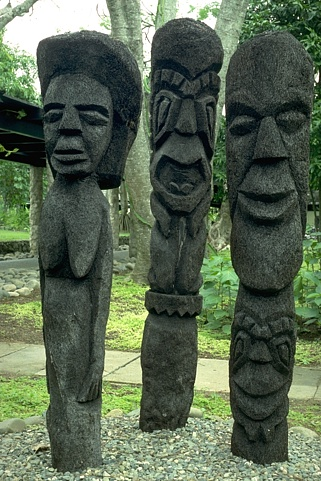
\includegraphics[width=0.29\textwidth]{images/examples/tikis/tikis.jpg}
}
\subfigure[Structured voting is a way of weighting oversegmentation contours]{%
 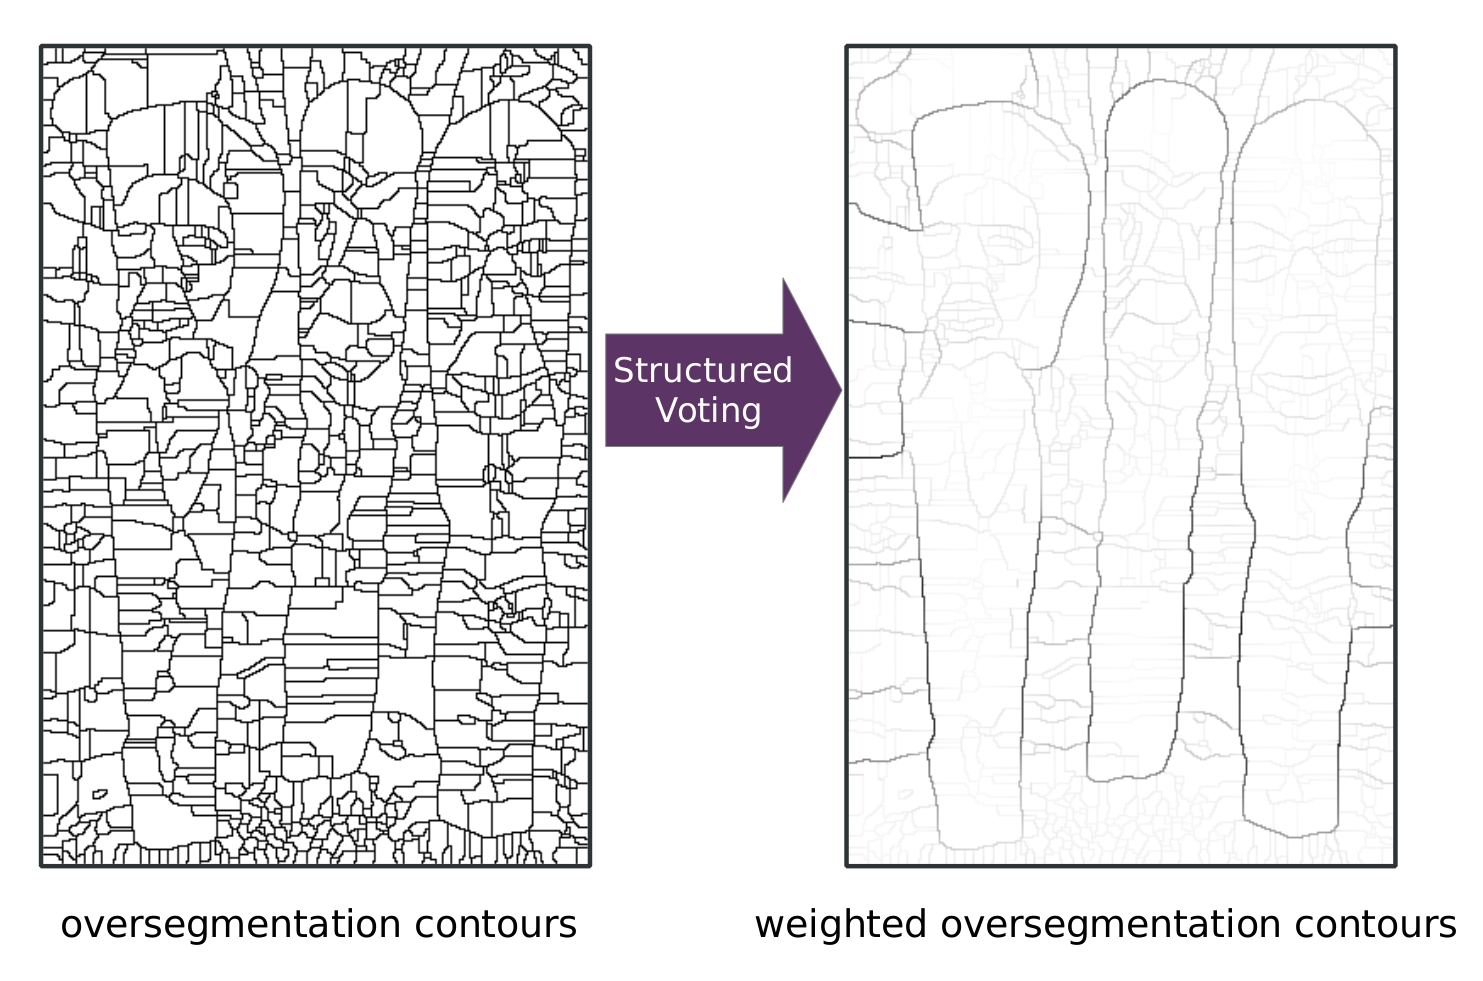
\includegraphics[width=0.66\textwidth,frame]{images/conclusions/weighting-oversegm-contours.png}
}
\caption[From edges to contours: a new approach]{We proposed a new approach for obtaining contours, given image edges.}
\label{fig:weighting-oversegm-contours}
\end{figure}

\section{Open questions} % be more positive - don't say 'Problems' :)
%While our 
Our best-performing experiments still narrowly miss on improving over the baseline that we defined ({\tt SE-OWT} in \sref{sec:ch5-SE-UCM-baseline}). That raises the question whether we can %hope to 
significantly improve on the current best achieved results using {\tt Structured voting}. Still, in the following we give directions for future work.

\subsection{Potential improvements}
% \section{Future work}

Analysing the ``voting'' strategy of {\tt SE} we remarked in \sref{sec:ch2-edge-detection} that each pixel receives $256$ binary votes. In comparison, applying % using %with 
our {\tt Structured voting} we vote only using %with 
patches {\it centred} on a watershed contour location, subsequently averaging the votes on the watershed arc. Our schema results in an order of magnitude less votes ($20$ to $40$). This discrepancy makes us reconsider %doubt 
the conclusions we drew from our initial experiment, which we described in \sref{sec:ch4-SE-SV-UCM_SV_details}. We interpreted our results as permitting % namely, that it permits 
us to only vote centred around a watershed pixel location. Two follow-up experiments can be performed:

\begin{enumerate}
 \item Modification of the experiment discussed in \sref{sec:ch4-SE-SV-UCM_SV_details}, where we first close edges into contours using a watershed transformation. Then we %subsequently 
 rerun the {\tt SE} with the patches cropped centred around a watershed location voting only on the underlying watershed arc (and not on all arcs that are inside the watershed patch, which is the case for the initial experiment in \sref{sec:ch4-SE-SV-UCM_SV_details}). If this experiment yields significant decay in edge extraction, that would mean our initial conclusion was fallacious.
 \item Modification of our {\tt Structured voting}, where we expand the voting scope. We should cast a vote not just on the underlying watershed arc, but on all watershed pixels within the patch which are also boundary pixels from the segmentation patch estimated by the decision tree. 
 Note that this is not a trivial experiment to conduct, since the locations of watershed contours will not necessarily coincide with the segmentation contours from the structured forest leaves. The votes on the watershed contours would therefore be scattered. % sparse 
 A strategy will need to be adopted to counter % poor 
 localisation mismatch between watershed contours and leaf segmentations. 
 If implemented correctly, we expect this experiment to show improved edge detection performance.
\end{enumerate}

Further, our {\tt SE-SV-UCM} uses the edge extractor {\tt SE} with baseline parameters: single scale detection, and without non-maxima suppression, see \sref{sec:ch5-nms-issue}. That means that the potential watershed locations are not as precisely % correctly 
localised as they would be, given %using %with 
a superior edge extractor. This explains the pronounced angular artefacts in the shape of the (non-weighted) oversegmentation contours that all our methods display before we conduct our {\tt Structured voting}. Our {\tt SV} relies on comparisons of small local patches (of size $16\times16$). Hence, it is logical that boundary localisation issues would thwart any metric that tries to compare two such patches. This matter is independent of the qualities of the scoring function {\it per se}. Although the BPR metric (see Section~\ref*{sec:ch4-boundary-and-region-metrics-maths}~\ref{par:ch4-BPR-maths}) can compensate for the inaccurate localisation, the choice of the distance parameter for the matching remains a problem. % regardless of the qualities of the metric per se.

\section{Conclusions}

\subsection{Patch transformations}

\textbf{A patch transformation is necessary:} As our experiments in Sections \ref{sec:ch5-superpixels-and-RI} and \ref{sec:ch5-naive-greedy-merge} show, directly comparing the oversegmentation patch (as is) to the structured forest patch is not beneficial. Instead, we simplify the watershed patch, striving %trying 
to keep only the information that is crucial to the boundary whose salience we attempt %want %try 
to evaluate. To this end, we experimented with a variety of patch transformations, see \fref{fig:patch-transformations}.

\begin{figure}[t]
\centering
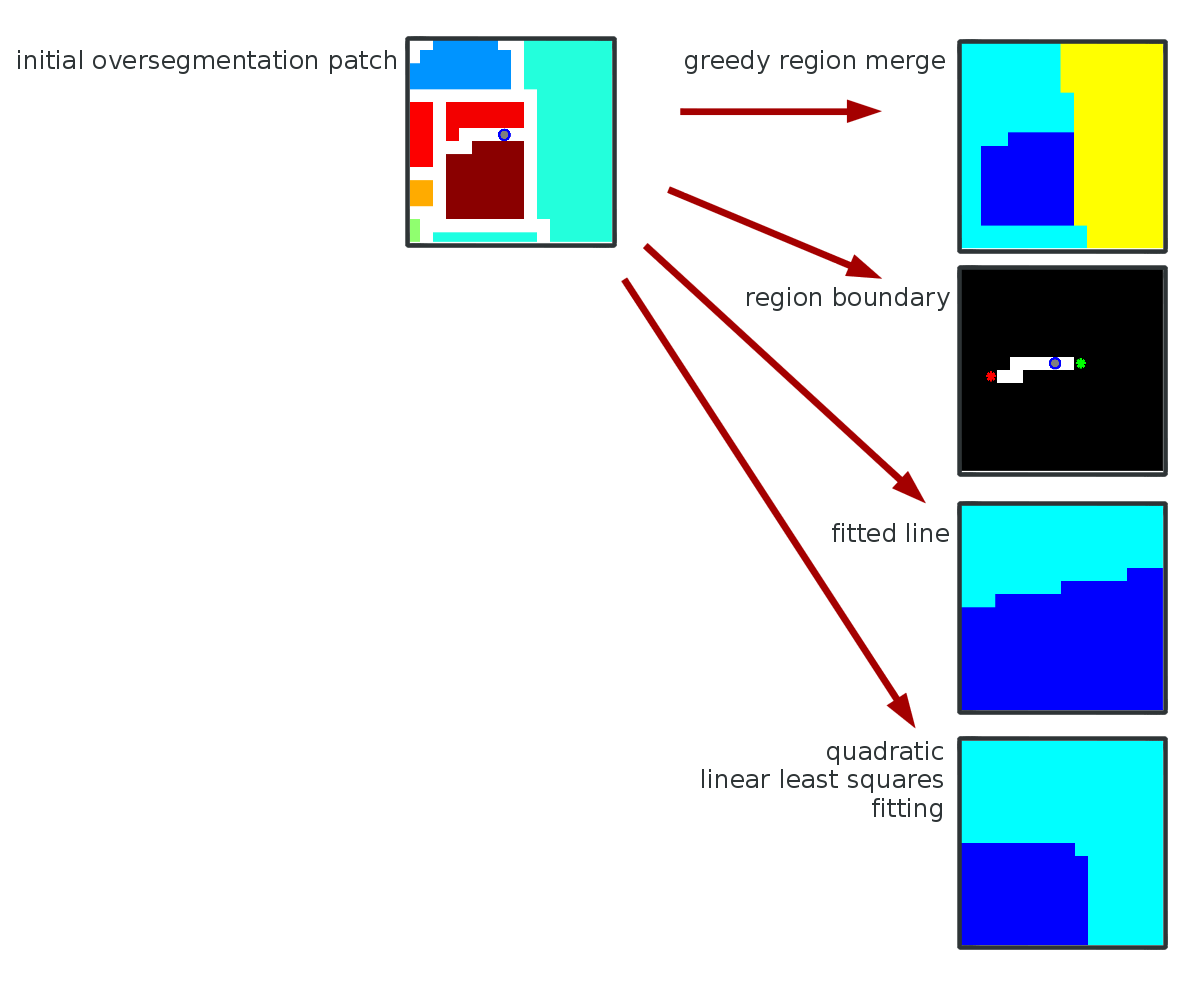
\includegraphics[width=0.6\textwidth]{images/conclusions/patch-transformations.png}
\caption[Proposed watershed patch transformations]{We propose, among others, the above patch transformations to simplify the watershed oversegmentation patch.}
\label{fig:patch-transformations}
\end{figure}

We obtain a ranking of the patch transformations. Overall, the quadratic linear least squares fitting (see \sref{sec:ch5-quadratic-fitting}) performs worst, since it is a complicated model and the fitted curves perceptually do not explain the data adequately. % satisfactorily. %very well. 
This model is followed by the na\"{\i}ve greedy merge, which cannot achieve good results because it excessively adapts to the segmentation estimated by the structured decision tree. All types of line fitting perform well with all our scoring functions (still, some scoring functions perform better, see \sref{sec:ch6-scoring-functions}).
% Since the quadratic model underperforms, we conclude that it is inadequate for the task.

\subsection{Scoring functions}
\label{sec:ch6-scoring-functions}
We analysed the theoretical properties of many boundary- and region-based metrics: Boundary Precision-Recall (BPR), Rand index (RI), Probabilistic Rand index (PRI), Segmentation covering (SC), Intersection over union (IoU), VPR not-normalised, and VPR normalised according to the ground truths, see \sref{sec:ch4-boundary-and-region-metrics-maths}. Further, we defined new metrics that we crafted to the %are suitable for the 
problem of small segmentation patches comparison for {\tt SV}: Rand Index Monte Carlo (RIMC) and VPR normalised according to the model capacity of the test segmentation. 

We experimented with the BPR, RI, RIMC, VPR not-normalised, VPR normalised according to the ground truths, and VPR normalised according to the model capacity of the test segmentation metrics, as most suitable for the task of structured patches comparison.

The BPR metric is the only metric applicable to compare the two patches in case of a ``watershed arc'' oversegmentation patch transformation, see Section~\ref*{sec:ch4-patch-transformations}~\ref{par:ch4-watershed-arc}.

Overall, the metric that we define based on the VPR: {\it VPR normalised according to the model capacity of the test segmentation}, displays 
the best performance. In retrospective this is not surprising since it provides normalisation for the often occurring case of a background segmentation patch estimated by the structured forest.

\subsection{Oracle case}
The oracle version of our pipeline allowed us to test the merits %quality 
of the different weighting strategies independent of the quality of the structured forest. Rather than using the forest's estimated patch predictions, we cropped patches from the human-annotated ground truths. The amount of improvement of the oracle case over the experiment, together with the overall oracle ranking were instrumental for interpreting our results. Importantly, the ranking of the oracle matches the ranking of the experiments, which verifies the correctness of the {\tt Structured voting} approach.

In conclusion, weighting strategies for {\tt Structured voting} are important. While we only researched a few dimensions that influence the performance of the method, we believe those are the most significant % instrumental, contributory, influential, important, critical, essential, pivotal, key
aspects that determine the output of our proposed pipeline {\tt SE-SV-UCM} for producing hierarchical image segmentations.
